\chapter{Revealing Object Interactions with \textsc{PathObjects}}
\chaptermark{Revealing Object Interactions}
\label{c:approach}

\section{Concept}

\section{Diagram Notation}
\subsection{Basic Concept}
\subsection{Diagram Aesthetics}
The object communication diagrams of \textsc{PathObjects} form graph structures, whereby  objects constitute nodes, and the arrows representing messages constitute edges.
Graph drawing is a research area with a long history of its own, and there is broad consent about the aesthetic properties that should be aimed at in order to maximize perceivability \cite{battista_graph_1998, kaufmann_drawing_2001, diehl_software_2007}.
Consequently, it stands to reason that these criteria should also be applied to our interactive object communication diagrams.
The seven most important criteria are presented in the following.

\paragraph{Crossing Minimization} User studies suggest that the most important aesthetic criterion is the minimization of edge crossings \cite{purchase_effective_2000, purchase_graph_2004, purchase_graph_2010}.
The more edges cross each other, the harder it becomes for the human eye to keep track of which nodes are connected by an edge.
Graph drawings that do not entail edge crossings are called planar, and are regarded as the best-case scenario.
But although planar graph drawing algorithms are comparatively simple, the excessive optimization of drawings in these premises will most likely interfere with other aesthetic criteria.

\paragraph{Bend Minimization} Bends make it harder for the human eye to follow the route of an edge.
Consequently, both the maximum number of bends on a single edge as well as the total number of bends on all edges should be as low as possible.
Furthermore, the variance of the number of bends on edges should be minimized.
However, recent studies suggest that continuity is more important than the number of bends \cite{diehl_software_2007}.

\paragraph{Length Minimization} Similar to crossings and bends, increasing edge lengths make it increasingly difficult for the viewer of a graph drawing to follow their paths.
Therefore, both the length of the longest edge and the total edge length should be minimized.
In addition, some authors state that the overall variance of lengths should be minimized in order to provide uniform edge lengths.

\paragraph{Area Minimization} The minimization of the area a diagram takes up is especially important when it cannot be scaled down arbitrarily.
This is the case with \textsc{PathObjects} diagrams, since textual information associated with nodes and edges has to stay above perceptive thresholds and may not overlap.
Furthermore, the efficient utilization of screen space is important.
Although our interactive information presentation offers scrolling functionality and thus allows diagram extents to exceed the viewport, scrolling interferes with reading the diagram and consequently complicates the assimilation of information.

\paragraph{Symmetry} Nodes should be distributed evenly on the canvas and thus should form a homogeneous density.
Furthermore, if the underlying graph structure features symmetries, these symmetries should also be reflected by the graph drawing.

\paragraph{Clustering} Interconnected parts of a graph should be drawn distinguishable from other so-called clusters.
In our case, connections are established through message exchanges, and objects or respectively nodes are connected stronger if they exchange more messages among each other than with other objects.
In addition, the edges between members of the same cluster should be shorter than edges that connect nodes from different clusters.

\paragraph{Orthogonality} Some authors state that fixing nodes and edges to an orthogonal grid improves the understandability of graph drawings \cite{sugiyama_methods_1981, batini_what_1985}.
And although Purchase et al. could not find significant evidence for this claim in a user study \cite{purchase_which_1997}, the majority of participants that were confronted with different variations of UML collaboration diagrams in another study nevertheless favored this edge routing strategy over other approaches \cite{purchase_graph_2004}.

Most of those drawing optimization criteria are NP-hard computational problems for tree structures \cite{battista_graph_1998}.
And since the graphs that should be presented through our interactive communication diagrams are call trees, this raises the question if the immediate character of the underlying tracing approach can be maintained.
For that reason, a runtime performance evaluation of the diagram construction is presented in Section \ref{s:DiscussionPerformance}.

So far, the presented aesthetic criteria are generally valid for all graph drawings regardless of their specific purpose.
In addition, Purchase et al. analyzed the user preferences and perceivability impacts of different variations of UML communication diagrams \cite{purchase_uml_2002, purchase_graph_2004}.
Since our interactive diagram notation is very similar to communication diagrams, the results of those studies also were taken into account.
\todo{blubb}

\subsection{Automatic Diagram Layout}
In general, there are many profound arguments for generating diagram layouts automatically.
For instance, automated drawing of diagrams has the side-effect that conformance to a certain style guide .
Furthermore, the costs of communication and thus the total costs of production and maintenance can be reduced by use of automated drawing of diagrams.
But the strongest reason to rely on the automated generation of diagram layouts becomes evident when taking the intended use of \textsc{PathTools} into account.


\section{Interactive Components}

\subsection{Navigation}
The implementation of the \textsc{PathObjects} concept for Squeak/Smalltalk offers three features that assist developers in navigating through an execution history.
First, the timeline gives an overview of all steps of the execution, or respectively the message sends and returns.
Second, the mini-map displays which objects are currently in the viewport, and which other objects also occur during the execution.
Third, the search bar allows developers to find classes, message sends, or specific instances

\subsubsection{Temporal Navigation}
\begin{figure}[tb]
	\centering
	
	\begin{subfigure}[b]{0.45\textwidth}
		\centering
        
\includegraphics[width=\textwidth]{../images/04-ImplTimeline1}
        \caption[Default View]{}
		\label{fig:ApproachTimelineDefault}
	\end{subfigure}
	\quad
	\begin{subfigure}[b]{0.45\textwidth}
		\centering
		
\includegraphics[width=\textwidth]{../images/04-ImplTimeline2}
		\caption[Search Result Highlighting]{}
		\label{fig:ApproachTimelineSearch}
	\end{subfigure}
	\quad
	\begin{subfigure}[b]{0.45\textwidth}
		\centering
		
\includegraphics[width=\textwidth]{../images/04-ImplTimeline3}
		\caption[Differing Metrics Applied to Item Height and Color]{}
		\label{fig:ApproachTimelineMetrics}
	\end{subfigure}
	
	\caption[Variations of the Timeline View]{Three variations of the timeline view that show the exact same execution history; in each case, the current step is highlighted and the according return point is marked in red.
		a) Default view with mapping of stack depth to item height.
		b) Search result highlighting.
		c) Differing metrics applied to item height and item color.
	}
	\label{fig:ApproachTimeline}
\end{figure}

Developers have to be enabled to navigate through the temporal dimension of execution traces.
On the one hand, stepwise forward and backward navigation should be facilitated.
On the other hand, it also should be possible to jump to specifics points of time in the execution history.
For these reasons, we propose an interactive diagram element, the so-called timeline.

Figure \ref{fig:ApproachTimeline} shows examples of the timeline view.
Each bar represents a step of the execution history, or respectively either a message send or the return from a message send.
The alignment along the horizontal axis corresponds to the chronological order of appearances.
The current step is marked with a blue overlay, and the corresponding send or return step is marked in red.
Developers can use the timeline to navigate through the execution history by either selection a specific step, by using the keyboard's left and right arrows, or by clicking the arrows that are displayed alongside the timeline.

All three examples in Figure \ref{fig:ApproachTimeline} show the exact same execution history at the exact same point of the execution.
Figure \ref{fig:ApproachTimelineDefault} represents the default configuration of the timeline view.
In this case, the height of the single timeline items corresponds to the depth of the call stack.
However, the concept of information layers (cf. \ref{??}\todo{cite}) allows to map arbitrary metrics to this dimension of the diagram.
Figure \ref{fig:ApproachTimelineSearch} shows how search results are highlighted within the timeline.
In the depicted example, the developer performed a search for occurrences of the \inlinecode{attach:} message.
Two matches are found, whereby each consists of a send and a returns step.
These occurrences correspond to the registration of the analog and digital clock instances at the clock timer.
Figure \ref{fig:ApproachTimelineMetrics} illustrates the usage of information layers in conjunction with the timeline view.
The height of the items now no longer represents the stack depth, but the number of variable accesses in each method.
The color of the items indicates the lines of code of each message.
One can see that the current step is the one with by far the most variable accesses.
Furthermore, the visualization indicates that most methods have an acceptable length, with the exception of the method that is the implementation of the selected message.

\subsubsection{Spatial Navigation}

\begin{figure}[tb]
	\centering
	
	\begin{subfigure}[b]{0.45\textwidth}
		\centering
		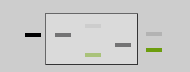
\includegraphics[width=\textwidth]{../images/04-ImplMinimap1}
		\caption[Default View]{}
		\label{fig:ApproachMinimapDefault}
	\end{subfigure}
	\quad
	\begin{subfigure}[b]{0.45\textwidth}
		\centering
		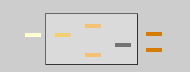
\includegraphics[width=\textwidth]{../images/04-ImplMinimap2}
		\caption[Application of Information Layers]{}
		\label{fig:ApproachMinimapMetric}
	\end{subfigure}
	
	\caption[Variations of the Mini-Map View]{a) Default configuration of the mini-map view; green represents objects that are involved in the current step, black and gray represent objects occurring in the past or future of the current execution history.
	
	b) \textsc{Fanin} metric applied to the color of objects; black indicates a high number of received messages.}
	\label{fig:ApproachMinimap}
\end{figure}

Contrary to temporal navigation, which allows to explore the chronological dimension of execution traces, developers also have to be enabled to navigate the spatial dimension of interactive communication diagrams.
For that reason, we suggest an interactive miniature representation of diagrams, the so-called mini-map.

The mini-map shows all objects that occur in a trace at a glance and allows to jump to any part of the canvas through mouse interactions.
Furthermore, it depicts which part of the canvas is currently displayed through a miniaturized viewport indicator.
Figure \ref{fig:ApproachMinimapDefault} depicts the default mini-map visualization.
All objects that are involved in the current step, either as sender, receiver, or argument of a message, are marked in green.
Objects that already occurred in the past of the execution history are depicted as black boxes.
Objects that did not occur up to the current step but will occur in future steps are marked in light gray.
Figure \ref{fig:ApproachMinimapMetric} represents an example how information layers can be applied to the mini-map.
In this case, the fan-in metric is mapped to the color of the object's representatives.
The heated-object scale indicates few received messages with light colors and the percipience of many messages in dark colors.
One can see that one object, namely the clock timer, receives more messages than any other object in this trace.

\subsubsection{Target-Oriented Navigation}
The spatial and temporal navigation components primarily support explorative approaches.
As opposed to this, developers also should be allowed to navigate to specific entities of interest provided that these entities are already known.
To make this possible, the third interactive navigation component of our communication diagrams is a search bar.

The search bar allows developers to find specific entities by reference to their name.
To simplify the process, entities that match a search term are shown and updated as the developer types.
The search functionality supports two different operational modes, namely precise and fuzzy search.
Fuzzy search performs a simple substring matching of the given input, and will return any class instance, class, or message whose name partly or fully matches the given search term.
For instance, this mode makes it possible to find all occurrences of instances of a specific class, by searching for \inlinecode{a ClassName} and omitting the object identifier, which as a matter of fact is part of an object name.
The precise mode, which is enabled as soon as the developer selects an entry from the list of suggested results, allows to search for specific classes, class instances, or messages.
For instance, this allows to search for all occurrences of a specific class.
This would not be possible with fuzzy search alone, since all instances of a class would always also match the search term and would thus lead to a cluttered search result.
As pointed out before, search results are indicated by highlighting timeline items (cf. Figure \ref{fig:ApproachTimelineSearch}).

\subsection{Exploration}
\subsection{Focusing}

\subsection{Information Layers}
Program comprehension usually does not end in itself but rather serves a specific purpose.
Consequently, the situations in which developers try to build an understanding of a software system are manifold.
Furthermore, different purposes require different additional information that can assist developers in specific situations.

For instance, if a developer wants to fix a defect, information such as recent changes that have been made to the system might be of interest.
Furthermore, one might want to display root cause probabilities along with methods.
In contrast, if the goal is a general refactoring to improve the overall code quality, one might be interested in metrics like lines of code or cyclomatic complexity.
The elimination of performance bottlenecks constitutes another common scenario.
In this case, developers most likely are interested in runtime profiling data.

At the same time, many dimensions of \textsc{PathObjects} diagrams are unused in the sense that they do not transport any semantic information.
The size of object nodes, the width of message connectors, the color and extent of timeline items, or the size and color of fonts constitute examples.
In addition, some facts are encoded redundantly.
For instance, objects that are somehow involved in the current step of the execution history are highlighted.
However, senders and receivers of messages are also clearly recognizable through  message connectors, and arguments and return values are flagged with role indicators.
Consequently, the color dimension of objects might also be used to encode additional information.

For these reasons, we propose the concept of information layers, which allow developers to project arbitrary metrics to various dimensions of \textsc{PathObjects} diagrams.
Thereby, metrics can provide data for messages, objects, or both.
Consequently, the dimensions that are supported for the visualization of a metric are dependent on the kind of data it provides.

\begin{table}[tb]
	\centering
	\footnotesize
	\begin{subtable}[t]{0.45\textwidth}
		\begin{tabular}{ll}
		\toprule[1.2pt]
		Message Metrics		& Dimensions 			\\
		\midrule
		Complexity			& Edge Color 			\\
		Last Change			& Edge Width			\\
		Lines of Code		& Timeline Item Color	\\
		Runtime Profiling	& Timeline Item Height	\\
		Stack Size			&						\\
		Variable Accesses	&						\\
		\bottomrule[1.2pt]
		\end{tabular}
		\caption[Message Metrics]{}
	\end{subtable}
	\qquad
	\begin{subtable}[t]{0.45\textwidth}
		\begin{tabular}{ll}
		\toprule[1.2pt]
		Object Metrics		& Dimensions 			\\
		\midrule
		\textsc{Fanin}		& Mini-Map Color		\\
		\textsc{Fanout}		& Object Color			\\
		\textsc{Faninout}	& Object Height			\\
		\hphantom{Runtime Profiling}	& Object Width			\\
							& \hphantom{Timeline Item Height} \\
							& \\
		\bottomrule[1.2pt]
		\end{tabular}
		\caption[Object Metrics]{}
	\end{subtable}
	\caption[Information Layers: Possible Metrics and Diagram Dimensions]{Possible (a) message and (b) object metrics that could be used as data source for information layers, together with the diagram dimensions they could be mapped to.}
	\label{t:ApproachLayers}
\end{table}